\usetikzlibrary {shapes.geometric}
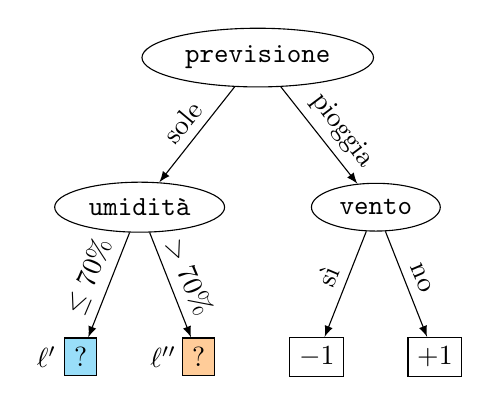
\begin{tikzpicture}[level distance=1.9cm,
    level 1/.style={sibling distance=3cm},
    level 2/.style={sibling distance=1.5cm},
    edge from parent/.style={draw,-latex}
]
    
    \node [ellipse,draw] {\texttt{previsione}}
        child {node[ellipse,draw] {\texttt{umidità}}
            child {
                node[rectangle,draw,fill=cyan!40] {?}
                node[xshift=-1.23em] {$\ell'$}
                edge from parent node[above,rotate=67] {$\leq 70\%$}
            }
            child {
                node[rectangle,draw,fill=orange!40] {?}
                node[xshift=-1.28em] {$\ell''$}
                edge from parent node[above,rotate=-67] {$> 70\%$}
            }
            edge from parent node[above,rotate=50] {sole}
        }
        child {node[ellipse,draw] {\texttt{vento}} 
            child {node[rectangle,draw] {$-1$} edge from parent node[above,rotate=67] {sì}}
            child {node[rectangle,draw] {$+1$} edge from parent node[above,rotate=-67] {no}}
            edge from parent node[above,yshift=-.3em,xshift=.2em,rotate=-53] {pioggia}
        };

\end{tikzpicture}